\documentclass[12pt, a4paper, openany]{book}
\usepackage[inline]{enumitem}
\usepackage{../generalStyle}

\graphicspath{ {./img/} }

\begin{document}

\title{Ricerca Operativa e Pianificazione delle Risorse}
\author{Fabio Ferrario}
\date{2022/2023}
\maketitle

\tableofcontents

\chapter{Introduzione}

\section{Il corso}
Il corso di ROPR verrà svolto da:
\begin{itemize}
    \item Fabio Antonio Stella
    \item Guglielmo Lulli
\end{itemize}

Il testo di riferimento è \emph{Frederick S. Hiller and Gerald J. Lieberman, Ricerca Operativa, McGraw-Hill, nona edizione, 2010.}


\section{Il programma}

\begin{itemize}
    \item Introduzione: storia-motivazione-esempi

    \item Ottimizzazione non lineare.
          \begin{enumerate}
              \item Ottimizzazione di funzioni non lineari ad una variabile: ricerca dicotomia-metodo Bisezione- metoto Newton.
              \item Ottimizzazione di funzioni non lineari multivariate: metodo Gradiente - metodo Newton
              \item Ottimizzazione non lineare vincolate: Condizioni di Karush-Kuhn-Tucker.
          \end{enumerate}
    \item Ottimizzazione lineare e intera.
          \begin{enumerate}
              \item Introduzione alla programmazione linare (PL): Proprietà dei problemi di PL, strategie di modellizzazione.
          \end{enumerate}
    \item Soft Computing per l'ottimizzazione.
\end{itemize}

\section{Modalità d'esame}
Due Modalità:
\begin{itemize}
    \item Modalità con Parziali
    \item Modalità con Scritto unico
\end{itemize}

\subsection*{Parziali}
Primo parziale sarà durante la settimana di sospensione didattica, il secondo a fine del corso a ridosso del primo appello completo.
Entrambe le prove hanno voto massimo 14 e soglia di superamento 6.
\\É possibile \emph{recuperare solo una delle due prove parziali}, a ridosso degli appelli completi.
\paragraph*{Assignments} Durante l'insegnamento verranno assegnati 4 Assignments da risolvere a casa e consegnare entro date stabilite,
Ad ogni assignment può andare un voto minimo di 0 a un massimo di 1.
\paragraph*{Orale} non obbligatorio, consiste in 3 domande (aperte/esercizi) su tutto il programma.
Si accede all'orale se si hanno già raggiunti i 18 punti. L'orale ha un voto di $\pm 3$.

\subsection*{Scritto unico}
Scritto (voto max 28) con domande/esercizi su tutto il programma.
Orale faoltativo si accede con un voto minimo di 15.



\chapter{Prerequisiti}
\section{Introduzione}
Per il corso di ROPR sono necessari alcuni prerequisiti, che verranno ripassati a lezione ma è bene conoscere già.
\\I prerequisiti indicati a lezione sono:
\begin{itemize}
    \item Familiarità con le \textbf{Funzioni}.
          \begin{itemize}
              \item Definizione di Funzione, dominio, codominio
              \item Definizione di F Suriettiva, iniettiva e biiettiva
              \item Definizione di F lineare/non lineare
              \item Definizione di F concava/convessa
          \end{itemize}
    \item Familiarità con gli \textbf{Spazi Vettoriali}.
          \begin{itemize}
              \item Definizione di Vettore, Spazio Vettoriale, Base di uno S. Vettoriale
              \item Definizione di vettori linearmente dipendenti/indipendenti
          \end{itemize}
    \item Familiarità con le \textbf{Matrici e Sistemi Lineari}.
          \begin{itemize}
              \item Definizione di matrice, rango e determinante
              \item Calcolo di una matrice inversa
              \item Definizione e risoluzione di un sistema lineare
          \end{itemize}
    \item Basi di \textbf{Topologia}.
    \item Basi di \textbf{Teoria dei Grafi}.
    \item Familiarità con il \textbf{Calcolo Differenziale}.
\end{itemize}
Un ripasso sui principali requisiti può essere trovato su E-Learning

\chapter{Modelli nella Ricerca Operativa}
\section{Problemi di Ottimizzazione}
La Ricerca Operativa si occupa di Problemi di Ottimizzazione:
\definizione{
    Data la funzione $f:\R^n \to \R$, un \textbf{problema di ottimizzazione} è formulabile come segue:
    $$\text{ opt } f(x) \text{ s.a. } x\in X, X\subseteq \R^n$$
    Dove \emph{opt} $\in \{min,max\}$ e \emph{s.a.} = "soggetto a".

}
I problemi di ottimizzazione possono essere:
\begin{itemize}
    \item Minimizzazione $min f(x)$
    \item Massimizzazione $max f(x)$
\end{itemize}
\definizione{
    In un problema di ottimizzazione la \emph{funzione} $f:R^n...$ è detta \textbf{funzione obiettivo},
    $X$ è la \textbf{regione ammissibile} e $x\in X$ sono le \textbf{variabili decisionali}.

}

Quindi un problema di ottimizzazione consiste nel determinare (se esistono) uno o più punti di \emph{min}/\emph{max} $x^*$ ($x^*$ è una particolare assegnazione che gode di una certa proprietà).

\paragraph*{Ottimizzazione Vincolata/non Vincolata}
Esistono due tipi principali di Ottimizzazione, determinate dall'esistenza o meno di delle \emph{regioni di vincolo}:
\begin{itemize}
    \item \textbf{Non Vincolata} $X = \R^n$: la ricerca dell'ottimo viene effettuata in tutto $R^n$.
    \item \textbf{Vincolata} $X \subset \R^n$: La ricerca dell'ottimo è soggetta al muoversi all'interno di una certa regione ($x \in [a, +\infty)$ per esempio).
\end{itemize}

Nel caso dell'ottimizzazione vincolata semplicemente si considera la regione dello spazio definita da un determinato intervallo,
quindi le soluzioni valide di solito cambiano.
\paragraph*{Ottimizzazione Intera e Binaria}
Non esiste solo l'ottimizzazione in cui le variabili assumono valori nello spazio reale, ma esistono anche ottimizzazioni con delle caratteristiche particolari.
\\Il vincolo $X\in Z^n$ richiede che le mie soluzioni \emph{siano valori interi}, quindi \textbf{ottimizzazione intera}.
\\Un altro vincolo molto "reale" è $x\in \{0,1\}^n$, in questo caso si chiama \textbf{ottimizzazione binaria} (vero falso, spento acceso,...).
Entrambe queste ottimizzazioni formano le ottimizzazioni a numeri interi.
Esiste anche l'ottimizzazione mista, in cui alcune variabili sono intere e altre binarie.

\section{Programmazione Matematica}
\definizione{
    Quando l'insieme delle soluzioni ammissibili di un problema di ottimizzazione viene espresso attraverso un sistema di equazioni e disequazioni,
    esso prende il nome di \emph{Programmazione Matematica}.
}
Ovvero, se i vincoli di un problema di ottimizzazione vengono espressi tramite delle equazioni/disequazioni, allora questo problema diventa un problema di programmazione matematica.

\subsection*{Come si definiscono i vincoli}
I vincoli vengono espressi con delle espressioni del tipo $g_i(x) \begin{cases}
        \geq \\ = \\ \leq %%sistemare questa dicitura
    \end{cases} 0$
in cui $g_i: X\to \R$ è una funzione generica che lega tra loro le variabili decisionali.
Nota che i vincoli dipendo dalle \emph{stesse variabili da cui dipende la funzione obiettivo}.
\\L'insieme (somma) di tutti i vincoli definisce la \emph{regione ammissibile}, se $x \in X$ allora è una soluzone ammissibile.
\\In un problema di ottimizzazione abbiamo quindi $m$ vincoli e $n$ variabili.

\paragraph*{Le possibilità} Quando risolviamo un problema di PM abbiamo quindi le seguenti possibilità:
\begin{itemize}
    \item Problema non ammissibile, $X = \emptyset$ (problema mal posto con regione ammissibile vuota)
    \item Problema illimitato, ovvero per ogni soluzione che trovo ne posso trovare un'altra che è MIGLIORE di quella che ho trovato, (può essere illim superiormente o infer)
    \item Problema con soluzione ottima unica
    \item Problema con più soluzioni ottime (anche infinite), tutte le ottime hanno lo stesso valore della funzione obiettivo.
\end{itemize}

\paragraph*{Ottimi Globali e Locali}
I punti di ottimo possono essere Locali o Globali (se la funzione è convessa Locale=Globale). NB un minimo globale è anche locale, un minimo locale non necessariamente è globale.
Ad oggi \emph{non} sappiamo dire se una soluzione sia Globale, sappiamo solo con certezza che sia locale (a meno di usare brute force).
\\La risoluzione di un problema di programmazione matematica consiste nel trovare una soluzione ammissibile che sia ottimo GLOBALE.
Alla fine della fiera la definizione di globale e locale corrisponde a quella di Analisi Matematica.
I punti di ottimo globali possono essere multipli.

\chapter{Metodo del Simplesso}
Il metodo del simplesso è una pocedura algebrica che si basa su dei \emph{concetti geometrici}.
\paragraph*{Alcuni Termini}
Questo metodo si basa su alcune terminologie che ci servono per capire come funziona.
Definiamo quindi:
\begin{itemize}
    \item \textbf{Frontiera del vincolo}: è la "linea" di demarcazione di un vincolo.
    \item \textbf{Vertice}: un vertice è un punto di intersezione di coppie di frontiere di vincoli.
          \begin{itemize}
              \item \textbf{Vertici Adiacenti}: Due vertici si dicono adiacenti se condividono $n-1$ frontiere di vincoli.
              \item \textbf{Spigolo}: segmento che collega due vertici adiacenti
          \end{itemize}
    \item \textbf{Vertice Ammissibile}: Un vertice è detto ammissibile se \emph{fa parte} della regione ammissibile
    \item \textbf{Vertice \emph{non} ammissibile}: Un vertice è detto \emph{non} ammissibile se \emph{non} fa parte della regione ammissibile.
\end{itemize}
\begin{center}
    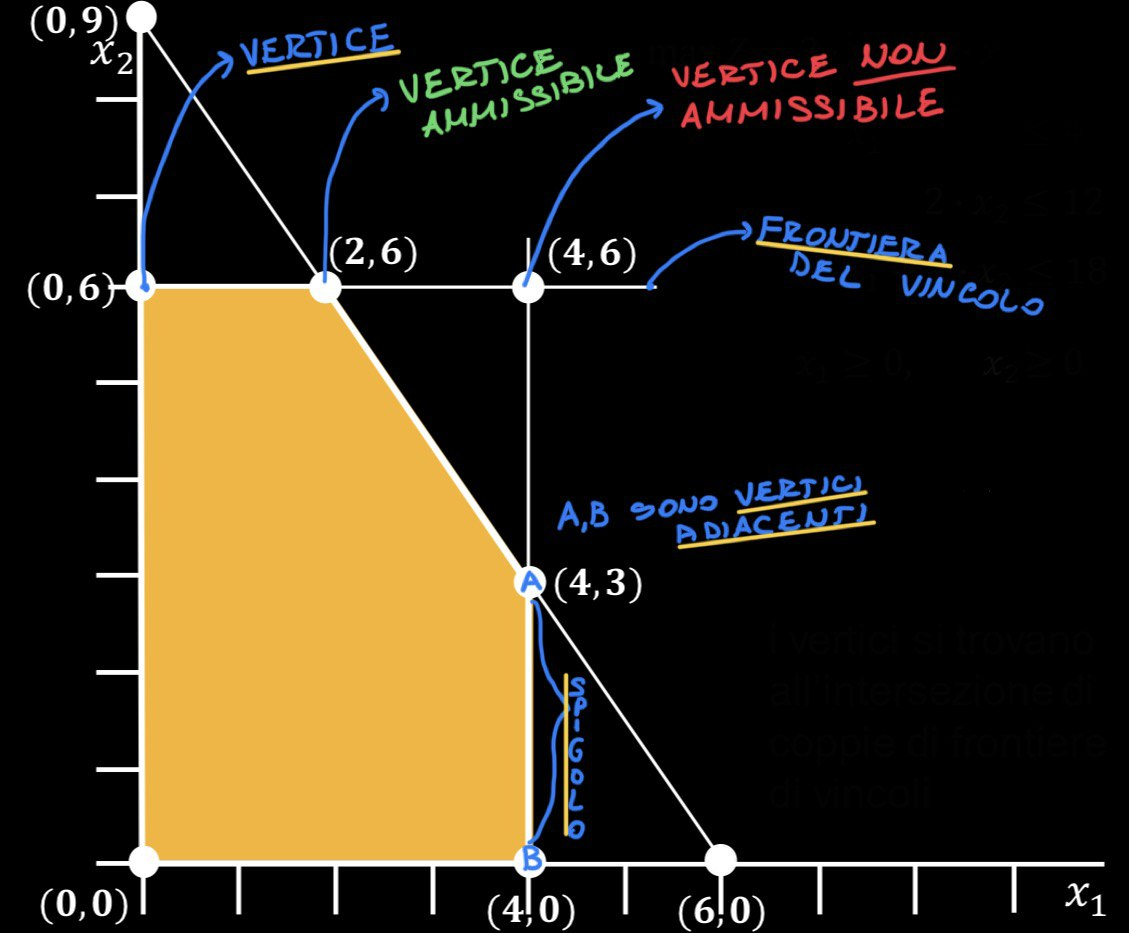
\includegraphics[width=0.8\textwidth]{img/Simplesso1.jpg}
\end{center}
\paragraph*{Test di Ottimalità}
L'interesse per i \emph{vertici adiacenti} sta nella seguente proprietà di cui godono:
\definizione{
    Si consideri ogni problema di PL tale da ammettere almeno una soluzione ottimale:
    \\Se una soluzione vertice non ammette soluzioni vertice a egli adiacenti con valore della funzione obiettivo
    migliore, allora la \textbf{soluzione} in questione è \textbf{ottimale}.
}

\section{La Procedura Algebrica}
Il metodo del simplesso è utilizzabile sia in forma algebrica che geometrica.
Siccome questo algoritmo è usualmente eseguito su un calcolatore, che è in grado di interpretare solo istruzioni algebriche,
è necessario tradurre la procedura geometrica in una procedura algebrica, che si basa sulla risoluzione di un sistema di equazioni lineari.
\paragraph*{Forma Aumentata}
Per usare il metodo del simplesso bisogna trasformare il modello dalla \emph{forma standard} alla \emph{forma aumentata}:
\\Per fare ciò bisogna fare le seguenti operazioni:
\begin{enumerate}
    \item Trasformo tutti i vincoli (tranne quelli di non negatività) in vincoli di \emph{eguaglianza}:
          $ x_1 +  x_2 \leq 5 \to  x_1 + x_2 = 5$
    \item Per ogni vincolo aggiungo una \textbf{Variabile di Slack}
          \\Ogni vincolo riceve una variabile di slack unica, quindi se abbiamo:
          \[
              \begin{cases}
                  x_1 \leq 3 \\
                  x_2 \leq 2 \\
                  x_1 + x_2 \leq 5
              \end{cases}
              \to
              \begin{cases}
                  x_1 + x_3 = 3 \\
                  x_2 + x_4= 2  \\
                  x_1 + x_2 + x_5 = 5
              \end{cases}
          \]
          $x_3,x_4,x_5$ sono le \emph{variabili di slack}.
          Assumendo che $x_1 = 0$, la variabile di slack $x_3$ è la \emph{quantità che manca al termine sinistro della diseguaglianza,
              affinchè questa sia verificata con il segno di uguaglianza }
\end{enumerate}
Le variabili di slack hanno alcune proprietà che sono utili da tenere a mente:
Per un qualunque valore delle variabili decisionali:
\begin{itemize}
    \item Se $slack = 0 \implies$ La soluzione corrispondente giace sulla frontiera del vincolo della forma originale.
    \item Se $slack > 0 \implies$ La soluzione corrispondente giace sul lato ammissibile della frontiera del vincolo della forma originale.
    \item Se $slack < 0 \implies$ La soluzione corrispondente giace sul lato NON ammissibile della frontiera del vincolo.
\end{itemize}
Si definisce \textbf{Soluzione Aumentata} una soluzione del modello in forma originale che viene \emph{aumentata} tramite i
corrispondenti valori delle variabili di slack.
\subparagraph*{Soluzione di Base}
Si definisce soluzione di base, un vertice del modello in forma aumentata.
\\Se abbiamo come variabili di base $x_1=4,x_2=6$ e come variabili di slack $x_2=0,x_3=0,x_4=-6$ allora la soluzione
di base (non ammissibile) associata sarà $(4,6,0,0,-6)$.
\subsection*{Variabili di Base e Non}
Un modello in forma aumentata consiste di $d$ variabili decisionali e $s$ variabili di slack.
Abbiamo quindi a disposizione $d$ gradi di libertà per risolvere il sistema lineare.
In altre parole, quando risolviamo un sistema lineare (ponendo a zero il valore di x variabili scelte arbitrariamente)
abbiamo tante variabili azzerabili quante sono le variabili decisionali.
\paragraph*{Soluzione di base}
Una \textbf{soluzione di base} gode delle seguenti proprietà:
\begin{enumerate} %Riformula per capire meglio
    \item Una variabile può essere \emph{Di base} o \emph{NON di base}
    \item Il numero delle variabili di base \emph{eguaglia il numero dei vincoli funzionali},
          Di conseguenza il numero delle variabili non di base eguaglia il numero totale delle variabili, meno il numero dei vincoli funzionali
    \item Le variabili NON di base \emph{vengono poste a zero}
    \item I valori delle variabili di base sono ottenuti come risoluzione simultanea del sistema di equazioni lineari (in forma aumentata).
    \item Se le variabili di base soddisfano i vincoli di non negatività, la soluzione di base è una soluzione ammissibile di base.
\end{enumerate}
\paragraph{Soluzioni di Base Adiacenti}
Due soluzioni di base ammissibili sono \emph{adiacenti} se sono caratterizzate dal \textbf{condividere le stesse variabili non di base eccetto una}.
\\Di conseguenza, muoversi da una soluzione di base ammissibile ad una soluzione ad essa adiacente
\emph{Implica che una variabile non di base divenga di base} e che \emph{una variabile di base divenga non di base}.
Il che richiede di aggiustare i valori delle variabili di base per garantire che il sistema di equazioni sia ancora soddisfatto.

\chapter{Dualità}
Ad ogni problema di programmazione lineare, che d'ora in poi chiameremo problema \textbf{Primale},
è associato un problema chiamato \textbf{Duale}.
La soluzione ottimale del problema Duale fornisce i \emph{prezzi ombra} del problema Primale.

\paragraph{Anailisi di Sensitività} La teoria della Dualità permette l'implementazione e interpretazione dell'analisi di sensitività.
\\L'Anaalisi di Sensitività è una tecnica che permette di decidere i valori di alcuni parametri di un problema di PL.

\section{Da Primale a Duale}
Un problema duale è strettamente legato al suo primale, infatti per passare da un problema al suo duale:

\begin{center}
    \begin{tabular}{ |c|c| }
        \hline
        max $c^T x $ & min $b^T \lambda $  \\
        $A x \leq b$ & $ A \lambda \geq c$ \\
        $x \geq 0$   & $ \lambda \geq 0 $ \\
        \hline
    \end{tabular}
\end{center}

In generale per passare da un primale a un duale valgono queste regole:

\begin{center}
    \begin{tabular}{ |l|c|c| }
        \hline
        Funzione Obiettivo:      & max $c_i^Tx$      & min $b^T\lambda$   \\
        \hline \hline
        Vincoli $\leq$ (primale) & $a_i^Tx \leq b_i$ & $\lambda_i \geq 0$ \\
        Vincoli $=$ (primale)    & $a_i^Tx = b_i$    & $\lambda_i$ Libera \\
        Vincoli $\geq$ (primale) & $a_i^Tx \geq b_i$ & $\lambda_i \leq 0$ \\
        \hline
        Vincoli Non negatività   & $x_j\geq 0$       & $A_j^T \geq c_j$   \\
        Variabile Libera         & $x_j$ Libera      & $A_j^T = c_j$      \\
        Vincoli Non positività   & $x_j\geq 0$       & $A_j^T \geq c_j$   \\
        \hline
    \end{tabular}
\end{center}
Quindi dato un qualunque problema di PL:
\begin{itemize}
    \item un problema di MAX diventa un problema di MIN.
    \item i coefficenti del primale diventano i termini noti del duale
    \item i termini noti del primale diventano coefficenti del duale.
    \item i coefficienti di variabile rimangono invariati
\end{itemize}
Si può notare che il Duale di un problema Duale è il suo primale, quindi un problema di minimizzazione diventa un problema di massimizzazione.

\end{document}
